% \documentclass[12pt]{article}

%%v helpful MIT exam schema, see http://www-math.mit.edu/~psh/exam/examdoc.pdf
 \documentclass[8pt]{exam} 
% \qformat{\textbf{Question \thequestion}\quad \thepoints\hfill } % Large depth to make space}
 \renewcommand{\thesubpart}{(\roman{subpart})}
 \renewcommand{\subpartlabel}{\thesubpart}
 \footer{}{}{Page \thepage\ de \numpages}
\addpoints
% \pointsinmargin
% \boxedpoints
\renewcommand{\questionshook}{\setlength{\itemsep}{0.2cm}}
\renewcommand{\partshook}{
	\setlength{\itemsep}{0.1cm}
}

\usepackage{cmbright}

\pagestyle{empty} %for handouts
\addtolength{\jot}{2em} % this makes all formulae a bit more spaced vertically for handouts
\setlength{\parindent}{0pt} %we're not writing a novel
%\renewcommand{\arraystretch}{2} %makes tables taller, so easier to write in

\usepackage[fleqn]{amsmath}
\usepackage{amssymb} %standard classy maths symbols
\usepackage[a4paper, margin=1in]{geometry} %makes it easy to specify where to put stuff on the page

\usepackage{siunitx} %v handy way of getting SI units to typeset correctly...
%\sisetup{locale = FR} %... and now it will use a comma for decimals

\usepackage[utf8]{inputenc}

\usepackage{tcolorbox} % basic but good package for boxes around text
\tcbset{colback=black!5!white}
% \usepackage{color} % colours
%\newcommand{\fillin}{\color{black!1!white}} %makes the text disappear
%\definecolor{fillin}{rgb} {1.00,1.00,1.00}
%\renewcommand{\fillin}{\color{blue}} \definecolor{fillin}{rgb} {0.00,0.00,1.00} %makes the filling in text appear (in blue)

%\usepackage{enumitem} % can change the labels on lists, items, enumerates

\usepackage{tikz, pgfplots} % interval diagrams, sets, etc.
\usetikzlibrary{calc,trees,positioning,arrows,fit,shapes}

\begin{document}

\textbf{Name:} \dotfill

\begin{center}
\textbf{Reminder :} The \textbf{slope} \emph{(pente)} is defined by the ratio
$\displaystyle \frac{\mbox{\emph{vertical change}}}{\mbox{\emph{horizontal change}}} \stackrel{\mbox{\tiny notation}}{=} \frac{\Delta y}{\Delta x} $
\end{center}

\begin{questions}

\question[9] Graphically determine the \textbf{y-intercept} \emph{(l'ordonnée à l'origine)}, the slope, and write down the algebraic expression for the following lines.

\begin{center}
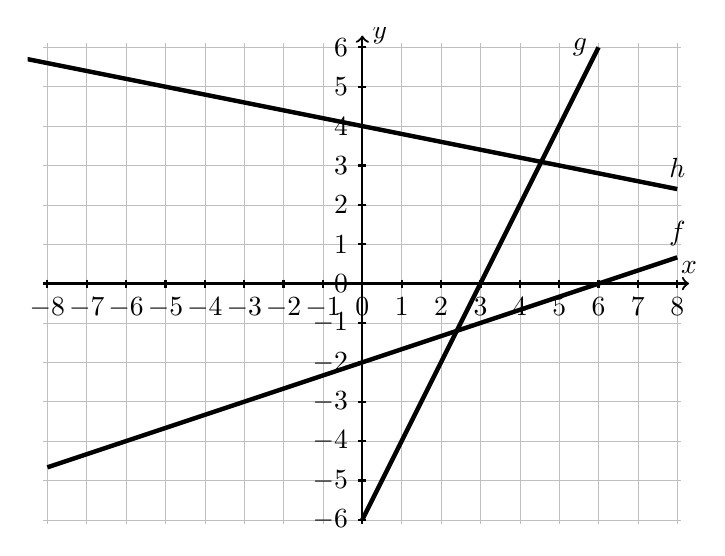
\begin{tikzpicture}[scale=0.5]
\clip (-8.5,-6.2) rectangle (8.5,6.5);
\draw[help lines, step=1, white!50!gray] (-8.1,-6.1) grid (8.1,6.1);
%\draw[help lines,line width=.8pt,step=1] (-0.1,-0.1) grid (10.1,10.1);

\draw[thick, ->] (-8.1,0) -- (8.3,0) node[above] {$x$};
\draw[thick, ->] (0,-6.1) -- (0,6.3) node[right] {$y$};

\foreach \x in {-8, -7, ..., 8}  \draw[thick] (\x,0.1) -- (\x,-0.1) node[below] {$\x$};
\foreach \y in {-6, -5, ..., 6}  \draw[thick] (0.1,\y) -- (-0.1, \y) node[left] {$\y$};

% Curve
\draw[ultra thick] plot[smooth, domain=-8:8] (\x, \x/3-2) node[above] {$f$};
\draw[ultra thick] plot[smooth, domain=0:6] (\x, 2*\x-6) node[left] {$g$};
\draw[ultra thick] plot[smooth, domain=-9:8] (\x, -\x/5+4) node[above] {$h$};

\end{tikzpicture}


\

\renewcommand{\arraystretch}{1.75}
\begin{tabular}{|c|c|c|c|}
\hline
function & y-intercept & \hspace{5mm} slope \hspace{5mm} & algebraic expression\\ \hline
$f$  & &   &  $f(x) = $ \hspace{5cm}      \\ \hline
$g$  & &   &    $g(x) = $   \hspace{5cm}    \\ \hline
$h$  &  &  &    $h(x) = $  \hspace{5cm}     \\ \hline
\end{tabular}
\end{center}

\

\question[3] Calculate the zeros of $f$ and $h$.
\fillwithdottedlines{21mm}

$$ f^{-1}(0) = \Bigg\{ \hspace{20mm} \Bigg\}, \qquad h^{-1}(0) = \Bigg\{ \hspace{20mm} \Bigg\}$$

\question[0] \textbf{Bonus.} Give the interval(s) where the functions $f$ and $h$ are \textbf{both} positive. 

\question[0] \textbf{Bonus.} Calculate the coordinates where the lines of $f$ and $h$ intersect.

\vfill

\end{questions}

\begin{tcolorbox}

\textbf{Nom de correcteur:}

\begin{center}
\gradetable[h][questions]
\end{center}

\end{tcolorbox}


\end{document}